%!TEX root = main.tex

\section{Decision procedure for $\strline_{\sf reg}$} \label{sec:decision}

The goal of this section is to prove Theorem~\ref{thm-main}, i.e., the decidability of the path feasibility of $\strline_{\sf reg}$. 
%is decidable in XXX. \zhilin{complexity should be added}
%

\subsection{The decision procedure}

We first show that semantically equivalent PSSTs can be effectively constructed from the $\extract$ and $\replaceall$ functions. 

\begin{lemma}\label{lem-str-fun-to-psst}
For each string function $f = \extract_{i,e}$, $\replace_{\pat, \rep}$, or $\replaceall_{\pat, \rep}$, a PSST $\cT_f$ can be constructed such that 
$$\cR_{f} = \{(w, w') \mid w'= f(w)\}.$$
\end{lemma}

%\begin{lemma}\label{lem-replace}
%A PSST $\cT_{\replace_{\pat, \rep}}$ (resp. $\cT_{\replaceall_{\pat, \rep}}$) can be constructed for $\replace_{\pat, \rep}$ (resp. $\replaceall_{\pat, \rep}$) such that $\cR_{\cT_{\replaceall_{\pat, \rep}}} = \{(w, w') \mid w'= \replaceall_{\pat, \rep}(w)\}$ (resp. $\cR_{\cT_{\replaceall_{\pat, \rep}}} = \{(w, w') \mid w'= \replaceall_{\pat, \rep}(w)\}$).
%\end{lemma}
%
The proof of Lemma~\ref{lem-str-fun-to-psst} is given in Appendix~\ref{appendix:sec-extract-replace-to-psst}.

With Lemma~\ref{lem-str-fun-to-psst}, the path feasibility of $\strline_{\sf reg}$ is reduced to the path feasibility of string-manipulating programs consisting of  a sequence of the statements of the form $z:=x \concat y$, $y:=\cT(x)$, and $\ASSERT{x \in \cA}$, where $\cT$ is a PSST and $\cA$ is an FA.  The class of programs is denoted by $\strline'_{\sf reg}$. We then  follow %the %backward computation %reasoning approach of 
the backward reasoning approach proposed in \cite{CCH+18,CHL+19} to solve the path feasibility of $\strline'_{\sf reg}$, where the key is to show that the pre-images of regular languages  under PSSTs  are regular and can be computed effectively.

\begin{definition}[Pre-image]
For a string relation $R \subseteq \Sigma^* \times (\Sigma^* \cup \{\nullchar\})$ and $L \subseteq \Sigma^*$, we define the \emph{pre-image} of $L$ under $R$ as $R^{-1}(L):=\{w \in \Sigma^* \mid \exists w'.\ w' \in L \mbox{ and } (w, w') \in R\}$. 
\end{definition}
 
\begin{lemma}[Pre-image of regular languages under PSSTs]
  \label{lem:psst_preimage}
  Given a PSST $\psst = (Q_T, \Sigma$, $X$, $\delta_T$, $\tau_T$, $E_T$,  $q_{0, T}$, $F_T$) and an \FA{} $\Aut
  = (Q_A, \Sigma, \delta_A, q_{0, A}, F_A)$, we can compute an \FA{} $\cB = (Q_B,
  \Sigma, \delta_B, q_{0, B}, F_B)$ in exponential time  such that $\Lang(\cB) = \cR^{-1}_{\cT}(\Lang(\Aut))$.
\end{lemma}

With Lemma~\ref{lem:psst_preimage}, we  solve the path feasibility of $\strline'_{\sf reg}$ by repeating the following procedure, until no more assignment statements are left. Let $S$ be the current $\strline'_{\sf reg}$ program.
\begin{itemize}
\item If the last assignment statement of $S$ is $y:=\cT(x)$, then let $\ASSERT{y \in \cA_1}$, $\cdots$, $\ASSERT{y \in \cA_n}$ be an enumeration of all the assertion statements for $y$ in $S$. Compute $\cR^{-1}_\cT(\Lang(\cA_1))$ as an FA $\cB_1$, $\cdots$, and $\cR^{-1}_\cT(\Lang(\cA_n))$ as $\cB_n$. Remove  the assignment  $y:=\cT(x)$ and add the assertion statements $\ASSERT{x \in \cB_1}$; $\cdots$; $\ASSERT{x \in \cB_n}$. 
%
\item If the last assignment statement of $S$ is $z:=x \concat y$, then let $\ASSERT{z \in \cA_1}$, $\cdots$, $\ASSERT{z \in \cA_n}$ be an enumeration of all the assertion statements for $z$ in $S$. Compute $\concat^{-1}(\Lang(\cA_1))$, the pre-image of $\concat$ under $\Lang(\cA_1)$, as a collection of FA pairs $(\cB_{1,j}, \cC_{1,j})_{j \in [m_1]}$, $\cdots$, and $\concat^{-1}(\Lang(\cA_n))$ as $(\cB_{n, j}, \cC_{n,j})_{j \in [m_n]}$ (c.f. \cite{CHL+19}). Remove the assignment $z:=x \concat y$, nondeterministically choose the indices $j_1 \in [m_1], \cdots, j_n \in [m_n]$, and add the assertion statements $\ASSERT{x \in \cB_{1,j_1}}; \ASSERT{y \in \cC_{1, j_1}}$; $\cdots$; $\ASSERT{x \in \cB_{n,j_n}}; \ASSERT{y \in \cC_{n, j_n}}$. 
\end{itemize}
Let $S'$ be the resulting $\strline'_{\sf reg}$ program containing no assignment statements. Then the path feasibility of $S'$ can be solved by checking the nonemptiness of the intersection of regular constraints for the input variables, which is known to be \pspace-complete \cite{Kozen77}.

\paragraph*{Complexity analysis.} Because the pre-image computation for each PSST incurs an exponential blow-up, the aforementioned decision procedure has a non-elementary complexity in the worst-case. Nevertheless, since the number of PSSTs is usually small in the path constraints of string-manipulating programs, the performance of the decision procedure is actually good on the benchmarks we tested, with the average running time per example less than one second (see Section~\ref{sect:impl}).


\begin{remark}
The aforementioned procedure extends the backward-reasoning approach in \cite{CCH+18,CHL+19}, since standard one-way and two-way finite-state transducers were considered therein and PSSTs, in particular priorities, are beyond them\footnote{It is known that deterministic streaming string transducers are expressively equivalent to two-way deterministic finite-state transducers, which, nevertheless, is not the case for nondeterministic transducers \cite{AC10,AD11}.}. 
%, PSSTs we introduce PSST, a new transducer model that covers the $\extract_{i,e}$ and $\replaceall_{\sf pat, rep}$ functions, where priorities are used to model the greedy/non-greedy semantics of $*$/$*?$ and string variables are used to store the matches of capturing groups. 
\end{remark}

%It remains to prove Lemma~\ref{lem-extract}-\ref{lem:psst_preimage}, which will be the focus of the next two subsections.
% in Section~\ref{sec-extract-replace-to-psst}-\ref{sec-pre-image}.



%%%%%%%%%%%%%%%%%%%%%%%%%%%%%%%%%%%%%%%%%%%%%%%
%\subsection{From $\extract$ and $\replaceall$ to PSST}\label{sec-extract-replace-to-psst}
%
%At first, we can adapt the pNFA construction in \cite{BDM14}, which in turn is a variant of the standard Thompson construction \cite{Thompson68}, and show the following result. 
%
%\begin{proposition}\label{prop-rwre-to-pfa}
%For each $\cgexp$ $e$, a PFA $\cA_e$ can be constructed in linear time such that 
%\begin{itemize}
%\item $\cA_e$ has a unique initial state without incoming transitions and a unique final state without outgoing transitions,
%%
%\item for subexpression $e'$ of $e$, $\cA_e$ contains an isomorphic copy of $\cA_{e'}$ (i.e. the PFA constructed for $e'$), denoted by ${\sf Sub}_{e'}[\cA_e]$. 
%\end{itemize}
%\end{proposition}
%%Let us use ${\sf Sub}_{e'}[\cA_e]$ to denote the isomorphic copy of $\cA_{e'}$ in $\cA_e$, as mentioned in Proposition~\ref{prop-rwre-to-pfa}.
%
%%
%%\begin{theorem}\label{thm-main}
%%The path feasibility of $\strline_{\sf reg}$ is decidable.
%%\end{theorem}
%%
%
%
%
%
%%\subsection{From $\regexp[\sf CG]$ to PFA}
%%\label{construction:pnfa}
%
%%\begin{figure*}
%%	\centering
%%	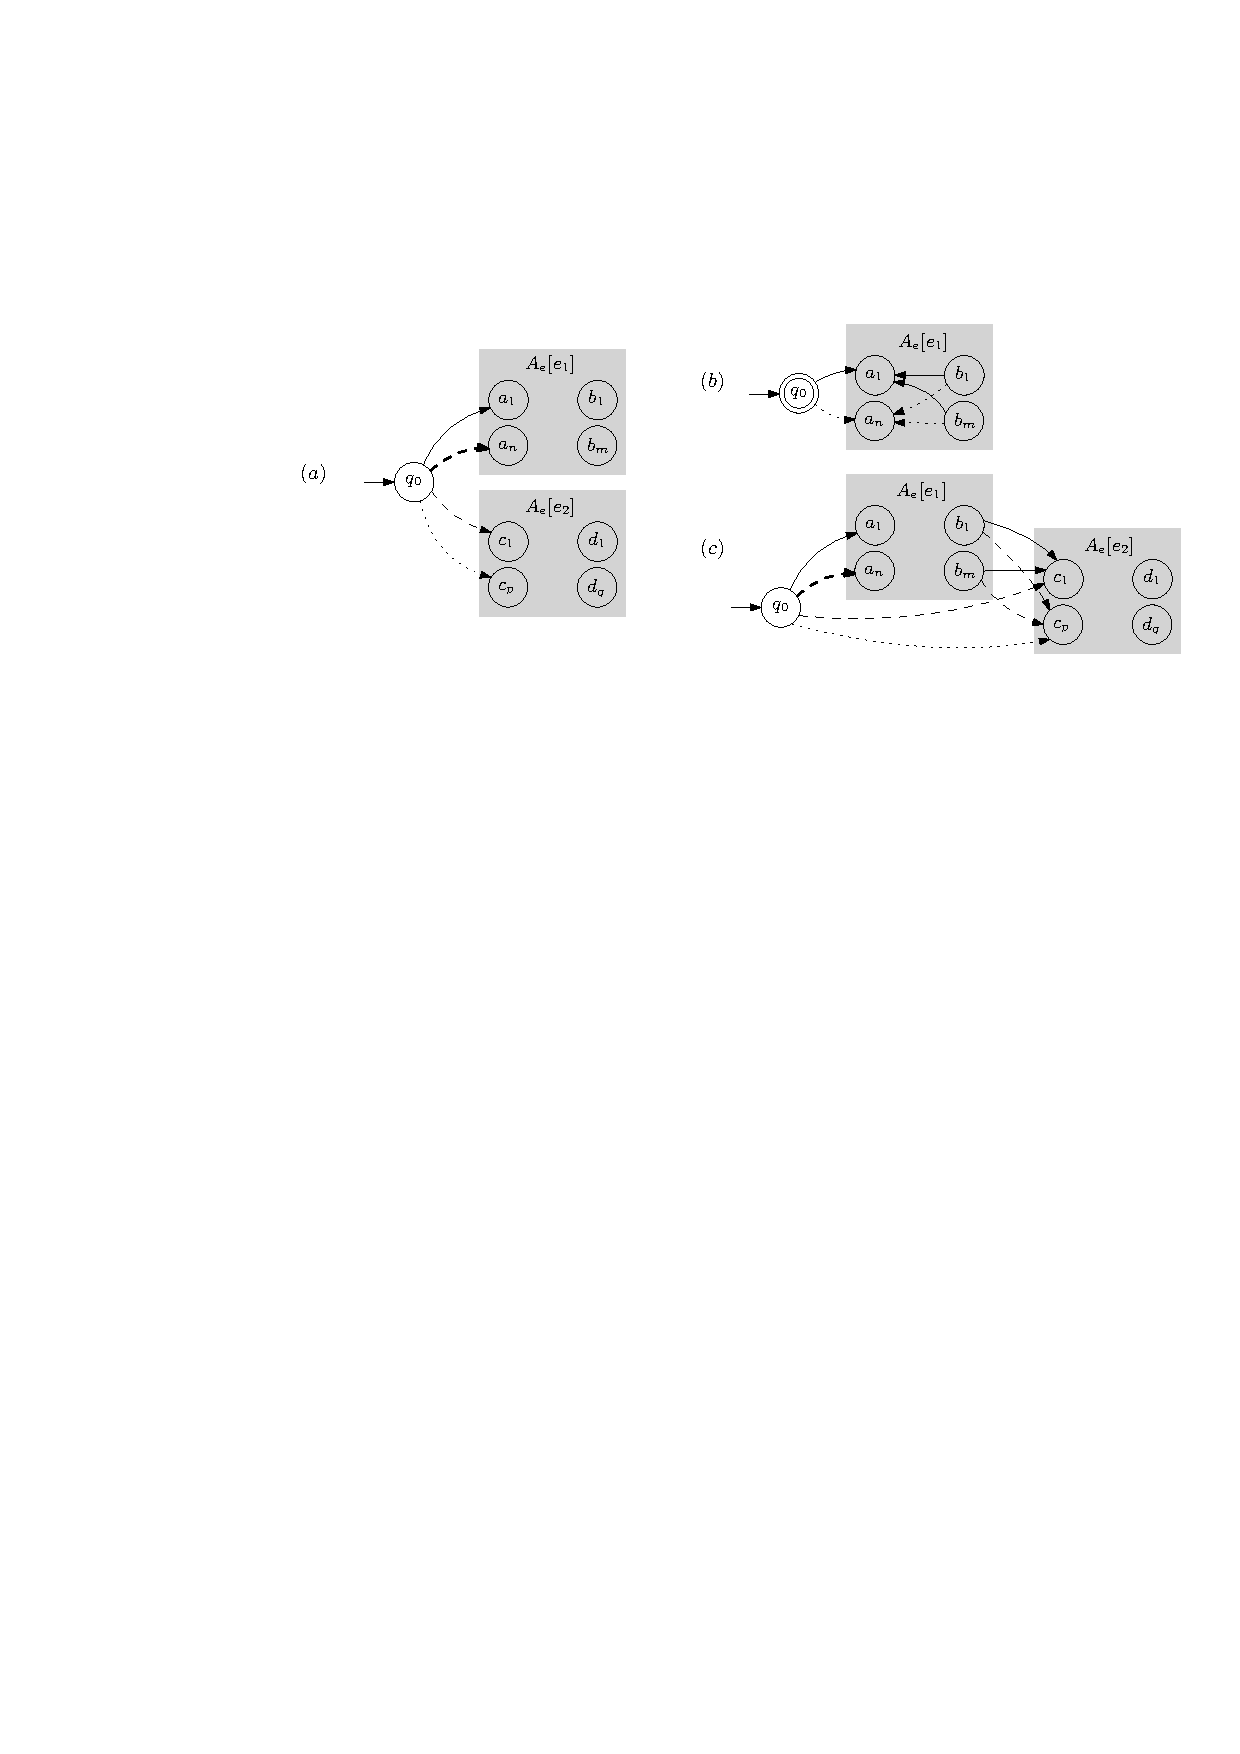
\includegraphics{pglushkov_01}
%%	\caption{pNFA $A_e$ for (a) $e=e_1+e_2$ (b) $e=e_1^{\ast}$ and (c) $e=e_1 \concat e_2$ where $\varepsilon \in \Lang(e_1)$ and $\varepsilon \notin \Lang(e_2)$. A transition of lower priority is depicted thiner and more densely dotted. }
%%	\label{fig:pglushkov}
%%\end{figure*}
%
%%For instance, if $e = (a (ab)^*)^*$ and $e' = a(ab)^*$, then $A_{e}[e']$ is the subgraph of $A_{e}$ comprising the states $\{a_1, a_2, b_3\}$ and the transitions $\{(a_1, a, a_2), (a_2, b, b_3), (b_3, a, a_2)\}$.
% 
%%Figure.\ref{fig:pglushkov} also illustrates the subgraphs corresponding to direct subexpressions of $e$.
%
%
%%\begin{definition}
%%Let $e \in \regexp[\sf CG]$ and $e'$ be a subexpression of $e$. Then a copy of $\cA_{e'}$ in $\cA_e = (Q, \Sigma, \delta, \tau, q_0, f_0)$ is a PFA $(Q', \Sigma, \delta', \tau', q'_0, f'_0)$ such that  
%%\begin{itemize}
%%\item $Q' \subseteq Q$, $q'_0, f'_0 \in Q'$, 
%%\item $\delta'$ is the restriction of $\delta$ to $Q'$, with the outgoing transitions of $f'_0$ removed, specifically, for every $\sigma \in \Sigma$ and $q \in Q' \setminus \{f'_0\}$, $\delta'(q, \sigma) = \delta(q, \sigma)$, $\tau'(q) = \tau(q)$, $\delta'(f'_0, \sigma) = ()$, and $\tau'(f'_0) = ((); ())$,
%%\item $(Q', \Sigma, \delta', \tau', q'_0, f'_0)$ is isomorphic to $\cA_{e'}$.
%%\end{itemize}
%%\end{definition}
%
%%From the aforementioned recursive construction of $\cA_e$, we know that for each subexpression $e'$ of $e$, a PFA for $e'$, which is isomorphic to $\cA_{e'}$, is also constructed. Let us use ${\sf Sub}_{e'}[\cA_e]$ to denote this PFA for $e'$, which, roughly speaking, is a subgraph of $\cA_e$.
%
%
%We are ready to prove Lemma~\ref{lem-extract} and Lemma~\ref{lem-replace}.
% 
%\begin{proof}[Lemma~\ref{lem-extract}]
%%\paragraph*{Construction of $\cT_{\extract_{i,e}}$.} 
%Let $e'$ be the subexpression corresponding to the $i$-th capturing group of $e$. In particular, if $i=0$, then $e' = e$. 
%Suppose $\cA_e = (Q, \Sigma, \delta, \tau, q_0, f_0)$. 
%%Moreover, let $\cA^\dag_e = (Q^\dag, \Sigma, \delta^\dag, \tau^\dag, q^\dag_0, f^\dag_0)$ be an isomorphic copy of $\cA_e$, where every state $q$ in $\cA_e$ is replaced by $q^\dag$ in $\cA^\dag_e$. Let us use ${\sf Sub}_{e'}[\cA^\dag_e]$ to denote the isomorphic copy of ${\sf Sub}_{e'}[\cA_e]$ in $\cA^\dag_e$.
%
%Intuitively, $\cT_{\extract_{i,e}}$ uses a string variable $x$ to store the value of the $i$th capturing group. Initially it assigns $\nullchar$ to $x$ to denote the fact that the capturing group is not matched yet. It then simulates $\cA_e$, and stores letters into $x$ when applying the transitions in ${\sf Sub}_{e'}[\cA_e]$. Finally, it outputs the value of $x$ when $\cA_e$ accepts.
%
%Formally, $\cT_{\extract_{i,e}} = (Q \cup \{q'_0\}, \Sigma, X, \delta', \tau', E', q'_0, F')$ (see Figure~\ref{fig-psst-extract}), where 
%\begin{itemize}
%\item $q'_0 \not \in Q$,
%%
%\item $X = \{x\}$,
%%
%%\item $\delta'$ is obtained from $\delta$ by adding $x: = x\sigma$ for each transition $(q, \sigma, q')$ in ${\sf Sub}_{e'}[\cA_e]$,  
%%
%\item $F'(f_0)= x$ and $F'(p)$ is undefined for all the other states $p \in Q  \cup \{q'_0\}$,
%%
%\item $\delta'$ and $\tau'$ are defined as follows,
%\begin{itemize}
%\item $\tau'(q'_0) = ((q_0); ())$,
%%
%\item $\delta'$ includes all the transitions in $\delta$,
%%
%\item $\tau'$ includes all the transitions in $\tau$,
%%
%\end{itemize}
%%
%\item $E'$ is defined as follows,
%\begin{itemize}
%\item if $q_0$ does not occur in ${\sf Sub}_{e'}[\cA_e]$, then $E'((q'_0, \varepsilon, q_0))(x) = \nullchar$, otherwise, $E'((q'_0, \varepsilon, q_0))(x) = \varepsilon$,
%%
%\item for each transition $(q, \sigma, q')$ in ${\sf Sub}_{e'}[\cA_e]$, $E'((q, \sigma, q'))(x) = x \sigma$,
%% 
%\item for each transition $(q, \sigma, q')$ such that $q$ does not occur not in ${\sf Sub}_{e'}[\cA_e]$ and $q'$ occurs in ${\sf Sub}_{e'}[\cA_e]$, $E'((q, \sigma, q'))(x) = \varepsilon$,
%%
%\item for all the other transitions $t$ of $\cA_e$, $E'(t)(x) = x$.
%\end{itemize}
%%
%%
%\end{itemize}
%
%\begin{figure}[ht]
%\centering
%%\rule{\linewidth}{0cm}
%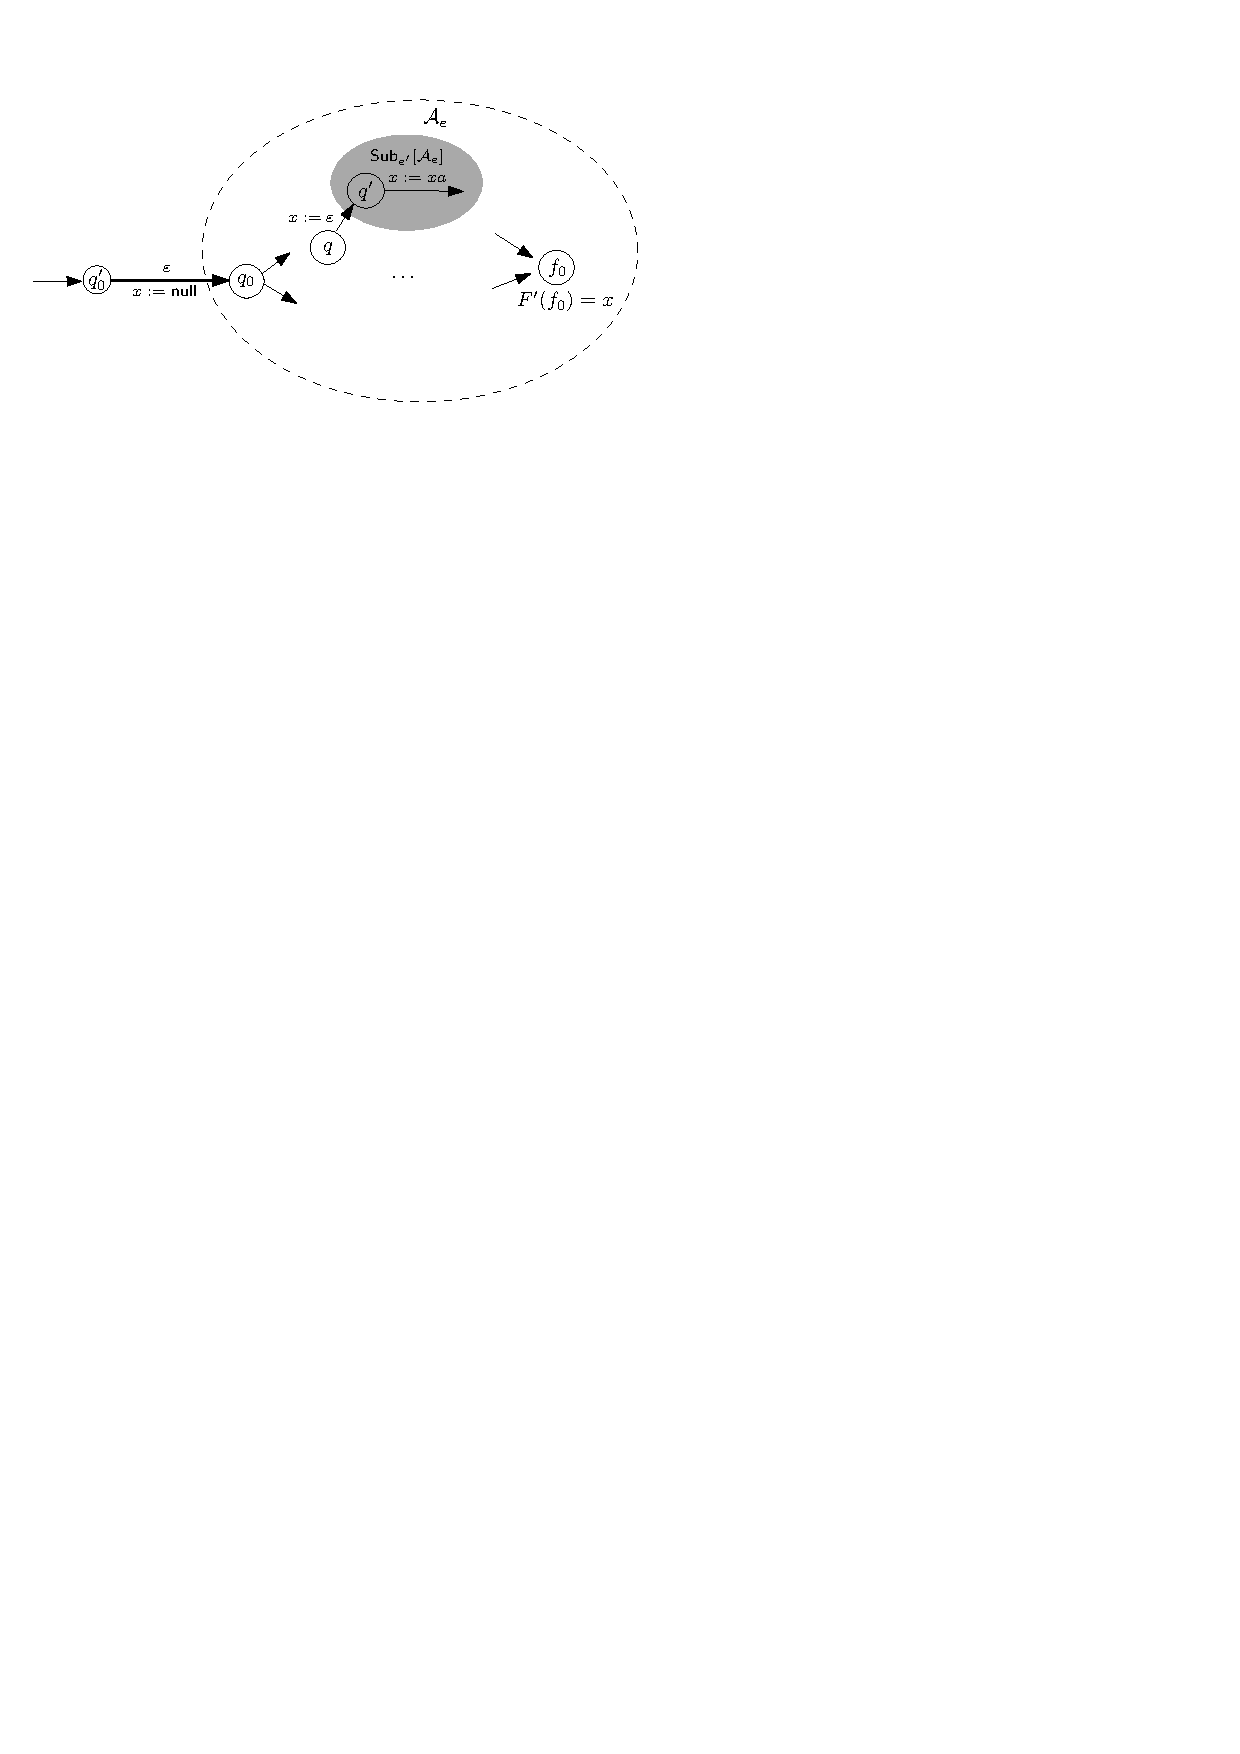
\includegraphics[width = 0.6\textwidth]{psst-extract.pdf}
%\caption{The PSST for $\extract_{i,e}$}
%\label{fig-psst-extract}
%\end{figure}
%\qed
%\end{proof}
%
%
%\begin{proof}[Lemma~\ref{lem-replace}]
%%\paragraph*{Construction of $\cT_{\replaceall_{\pat, \rep}}$.} 
%Let $\$i_1, \cdots, \$i_k$ with $i_1 < \cdots < i_k$ be an enumeration of all the references in $\rep$. 
%Moreover, for every $j \in [k]$, let $e'_{i_j}$ be the subexpression of $\pat$ corresponding to the $i_j$-th capturing group.
%
%Suppose $\cA_\pat = (Q, \Sigma, \delta, \tau, q_0, f_0)$. Then $\cT_{\replace_{\pat,\rep}}$ is obtained from $\cA_\pat$ by adding a fresh states $q'_0$ such that (see Figure~\ref{fig-psst-replace})
%\begin{itemize}
%\item $\cT_{\replace_{\pat,\rep}}$ goes from $q'_0$ to $q_0$ via an $\varepsilon$-transition of higher priority than the non-$\varepsilon$-transitions, in order to search the first match of $\pat$ starting from the current position, 
%%
%\item when $\cT_{\replace_{\pat,\rep}}$ stays at $q'_0$, it keeps appending the current letter to the end of $x_0$, 
%%
%\item starting from $q_0$, $\cT_{\replace_{\pat,\rep}}$ simulates $\cA_\pat$ and stores the matches of the $\$i_1$-th, $\ldots$, $\$i_k$-th capturing groups of $\pat$ into the string variables $x_1, \cdots, x_k$ respectively,   
%%
%\item when the first match of $\pat$ is found, $\cT_{\replace_{\pat,\rep}}$ goes from $f_0$ to $q'_0$ via an $\varepsilon$-transition, appends the replacement string, which is $\rep[x_1/\$_{i_1}, \cdots, x_k/\$_{i_k}]$, to the end of $x_0$, and keeps searching for the next match of $\pat$.
%\end{itemize}
%
%\begin{figure}[ht]
%\centering
%%\rule{\linewidth}{0cm}
%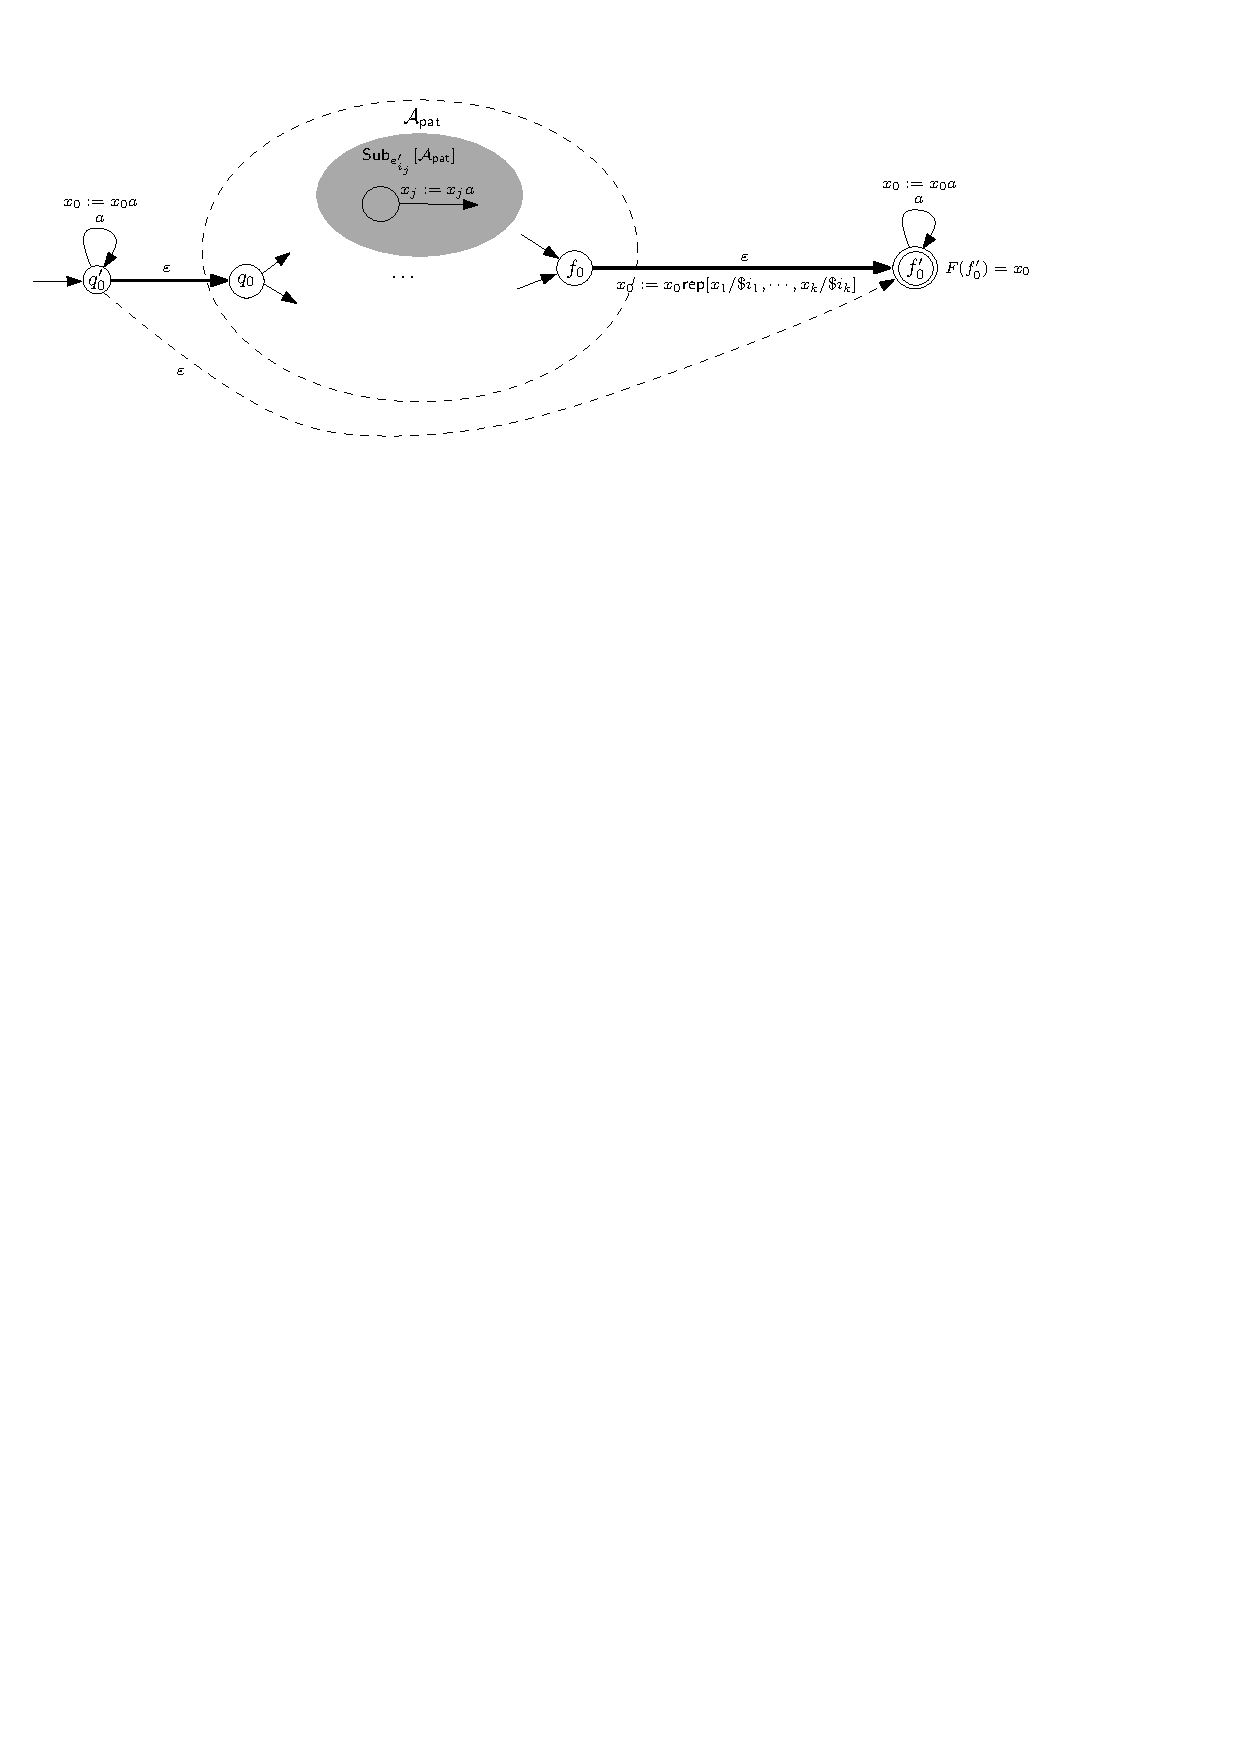
\includegraphics[scale=0.8]{psst-replace.pdf}
%\caption{The PSST for $\replace_{\pat,\rep}$}
%\label{fig-psst-replace}
%\end{figure}
%
%Formally, $\cT_{\replaceall_{\pat, \rep}} =$ $(Q \cup \{q'_0\}$, $\Sigma$, $X$, $\delta'$, $\tau', E, q'_0, F)$ where
%\begin{itemize}
%\item $q'_0 \not \in Q$,
%
%\item  $X = \{x_0, x_1, \cdots, x_k\}$,
%%
%\item $F(q'_0) = x_0$, and $F(q')$ is undefined for every $q' \in Q$,
%%
%\item $\delta'$ and $\tau'$ are obtained from $\delta$ and $\tau$ as follows,
%\begin{itemize}
%\item $\delta'(q'_0, \sigma) = (q'_0)$ for every $\sigma \in \Sigma$, and $\tau'(q'_0) = ((q_0); ())$,
%%
%\item for every $q \in Q \setminus \{f_0\}$ and $\sigma \in \Sigma$, $\delta'(q, \sigma) = \delta(q, \sigma)$ and $\tau'(q) = \tau(q)$, 
%%
%\item $\delta'(f_0, \sigma) = ()$ for every $\sigma \in \Sigma$ and $\tau'(f_0) = ((q'_0); ())$,
%\end{itemize}
%%
%\item $E$ is defined as follows, 
%\begin{itemize}
%\item for every transition $(q, \sigma, q')$ with $\sigma \in \Sigma^\varepsilon$ in $\cA_\pat$, $E(q, \sigma, q')(x_0) = x_0$,
%%
%\item for every transition $(q, \sigma, q')$ with $\sigma \in \Sigma^\varepsilon$ and $j \in [k]$,  if $(q, \sigma, q')$ occurs in ${\sf Sub}_{e'_{i_j}}[\cA_\pat]$, then $E(q, \sigma, q')(x_j) = x_j\sigma$, otherwise, $E(q, \sigma, q')(x_j) = x_j$,
%%
%%\item for all the other transitions $(q, \sigma, q')$ with $\sigma \in \Sigma^\varepsilon$ in $\cA_e$, we have $E(q, \sigma, q')(x) = x$, 
%%
%\item  for every $\sigma \in \Sigma$ and $j \in [k]$, $E(q'_0, \sigma, q'_0)(x_0) = x_0\sigma$ and $E(q'_0, \sigma, q'_0)$$(x_j) = x_j$, 
%
%\item $E(q'_0, \varepsilon, q_0)(x_j) = x_j$ for every $j \in [k] \cup \{0\}$, 
%%
%\item $E(f_0, \varepsilon, q'_0)(x_0) = x_0 \rep[x_1/\$i_1,\ldots, x_k/\$i_k]$, and for every $j \in [k]$, we have $E(f_0, \varepsilon, q'_0)(x_j) = \varepsilon$.
%
%\end{itemize}
%%
%\end{itemize}
%\qed
%\end{proof}

In the rest of this section, we are going to illustrate how to prove Lemma~\ref{lem:psst_preimage}, namely, how to compute the pre-images of regular languages under PSSTs.

\subsection{Computing the pre-image of regular languages under PSSTs}\label{sec-pre-image}

%In this subsection, we are going to show Lemma~\ref{lem:psst_preimage}, namely, how to compute the pre-images of regular languages under PSSTs.

%\tl{another way is to first define B as a PFA, could make the construction a bit modular?}\zhilin{Add a counter example for this natural idea.}
 
Let $\psst = (Q_T, \Sigma$, $X, \delta_T, \tau_T, E_T,  q_{0, T}, F_T)$ be a PSST  and $\Aut
  = (Q_A, \Sigma$, $\delta_A$, $q_{0, A}$, $F_A)$ be an \FA{}. Without loss of generality, we assume that $\Aut$ contains no $\varepsilon$-transitions. For convenience, we use $\cE(\tau_T)$ to denote $\{(q, q') \mid q' \in \tau_T(q)\}$. 

To illustrate the intuition of the proof of Lemma~\ref{lem:psst_preimage}, let us start with the following natural idea of firstly constructing a PFA $\cB$ for the pre-image: $\cB$ simulates a run of $\psst$ on $w$, and, for each $x \in X$, records an $\Aut$-abstraction of the string stored in $x$, that is, the set of state pairs $(p, q) \in Q_A \times Q_A$ such that starting from $p$, $\Aut$ can reach $q$ after reading the string stored in $x$. Specifically, the states of $\cB$ are of the form $(q, \rho)$ with $q \in Q$ and $\rho \in (\cP(Q_A \times Q_A ))^{X}$. Moreover, the priorities of $\cB$ inherit those of $\psst$. The PFA $\cB$ is then transformed to an equivalent FA by simply dropping all priorities. We refer to this FA as $\cB'$.

Nevertheless, it turns out that this construction is flawed: A string $w$ is in $\cR^{-1}_{\cT}(\Lang(\Aut))$ iff the (unique) accepting run of $\cT$ on $w$ produces an output $w'$ that is accepted by $\Aut$. However, a string $w$ is accepted by $\cB'$ iff \emph{there is a run of $\cT$ on $w$, not necessarily of the highest priority}, producing an output $w'$ that is accepted by $\Aut$. The following example illustrates the flaw of the construction above.

\begin{example}
\label{pre-image-count-examp}
Let $\cT_{\tt extract_{decimalReg,1}}$ be the PSST in Fig.~\ref{fig-psst-exmp} and $\cA$ be the FA corresponding to the regular expression $\{1,\cdots,9\}^*$, specifically, $\cA= (\{p_0\}$, $\{0,\cdots,9\}$, $\delta_A$, $p_0, \{p_0\})$, where $\delta_A = \{(q_0, \ell, q_0) \mid \ell = 1, \cdots, 9\}$.
%  in Figure~\ref{fig-pre-image-count-exmp}, that is, 
%\begin{itemize}
%\item $\cT=(\{q_0, q_1, q_2\}, \{a,b,c\}, \{x_0\}, \delta_T, \tau_T, E_T, q_0, F_T)$, where $\delta_T(q_0, \sigma) = (q_0)$, $\delta_T(q_1, a) = (q_1)$, $\delta_T(q_2, \sigma) = (q_2)$, $\tau_T(q_0) = ((q_1); ())$, $\tau_T(q_1)=((q_0, q_2);())$, and $\tau_T(q_2)= ((); ())$, $E_T(q_0, \sigma, q_0) (x_0) = x_0 \sigma$, $E_T(q_1, \varepsilon, q_0) (x_0) = x_0 c$, $E_T(q_1, \varepsilon, q_2) (x_0) = x_0 c$, $E_T(q_2, \sigma, q_2) (x_0) = x_0 \sigma$, for $\sigma \in\{ a, b\}$. Moreover, $F_T(q_2)= x_0$;
%
%\item $\cA = (\{p_0\}, \{a,b,c\}, \delta_A, p_0, \{p_0\})$, where $\delta_A$ = $\{(p_0, \sigma, p_0)$ $\mid \sigma = b, c\}$.
%\end{itemize}

Let us consider $w = 10$. The accepting run of $\cT_{\tt extract_{decimalReg,1}}$ on $w$ is $q_0 \xrightarrow[x_1:=x_11]{1} q_1 \xrightarrow[x_1:=x_10]{0} q_1 \xrightarrow{\varepsilon} q_2 \xrightarrow{\varepsilon} q_3 \xrightarrow{\varepsilon} q_4 \xrightarrow{\varepsilon} q_5 \xrightarrow{\varepsilon} q_6$, producing an output $10 \not \in \Lang(\cA)$. Therefore, $10 \not \in \cR_\cT^{-1}(\Lang(\cA))$. Nevertheless, if we consider the FA $\cB'$ constructed from $\cT$ and $\cA$,  it turns out that $\cB'$ does accept $w$, witnessed by the run $(q_0, \{(p_0,p_0)\}) \xrightarrow{1} (q_1, \{(p_0, p_0)\}) \xrightarrow{\varepsilon} (q_2, \{(p_0, p_0)\}) \xrightarrow{\varepsilon}  (q_3, \{(p_0, p_0)\}) \xrightarrow{\varepsilon}  (q_4, \{(p_0, p_0)\}) \xrightarrow{\varepsilon}  (q_5, \{(p_0, p_0)\}) \xrightarrow{0}  (q_5, \{(p_0, p_0)\}) \xrightarrow{\varepsilon}  (q_6, \{(p_0, p_0)\})$, where $\{(p_0, p_0)\}$ is the $\cA$-abstraction of the strings $\varepsilon$ and $1$. On the other hand, the run of $\cB'$ corresponding to the accepting run of $\cT$ on $w$, i.e. $(q_0, \{(p_0, p_0)\}) \xrightarrow{1} (q_1, \{(p_0, p_0)\}) \xrightarrow{0} (q_1, \emptyset) \xrightarrow{\varepsilon}  (q_2, \emptyset) \xrightarrow{\varepsilon} (q_3, \emptyset) \xrightarrow{\varepsilon} (q_4, \emptyset) \xrightarrow{\varepsilon} (q_5, \emptyset) \xrightarrow{\varepsilon} (q_6, \emptyset)$, is not accepting, where $\{(p_0,p_0)\}$ is the $\cA$-abstraction of $\varepsilon$ as well as $1$, and $\emptyset$ is the $\cA$-abstraction of $10$.
\end{example}

%%%%%%%%%%%%%%%%%%%%%%%%%%%%%%
%%%%%%%%%%%%%%%%%%%%%%%%%%%%%%
\hide{
\begin{example}
\label{pre-image-count-examp}
Let $\cT$ be the PSST and $\cA$ be the FA in Figure~\ref{fig-pre-image-count-exmp}, that is, 
\begin{itemize}
\item $\cT=(\{q_0, q_1, q_2\}, \{a,b,c\}, \{x_0\}, \delta_T, \tau_T, E_T, q_0, F_T)$, where $\delta_T(q_0, \sigma) = (q_0)$, $\delta_T(q_1, a) = (q_1)$, $\delta_T(q_2, \sigma) = (q_2)$, $\tau_T(q_0) = ((q_1); ())$, $\tau_T(q_1)=((q_0, q_2);())$, and $\tau_T(q_2)= ((); ())$, $E_T(q_0, \sigma, q_0) (x_0) = x_0 \sigma$, $E_T(q_1, \varepsilon, q_0) (x_0) = x_0 c$, $E_T(q_1, \varepsilon, q_2) (x_0) = x_0 c$, $E_T(q_2, \sigma, q_2) (x_0) = x_0 \sigma$, for $\sigma \in\{ a, b\}$. Moreover, $F_T(q_2)= x_0$;
%
\item $\cA = (\{p_0\}, \{a,b,c\}, \delta_A, p_0, \{p_0\})$, where $\delta_A$ = $\{(p_0, \sigma, p_0)$ $\mid \sigma = b, c\}$.
\end{itemize}

Let us consider $w = a$. The accepting run of $\cT$ on $w$ is $q_0 \xrightarrow{\varepsilon} q_1 \xrightarrow[x_0:=x_0c]{\varepsilon} q_0 \xrightarrow[x_0:=x_0a]{a} q_0 \xrightarrow{\varepsilon} q_1 \xrightarrow[x_0:=x_0c]{\varepsilon} q_2$, producing an output $cac \not \in \Lang(\cA)$. Therefore, $a \not \in \cR_\cT^{-1}(\Lang(\cA))$. Nevertheless, if we consider the FA $\cB'$ constructed from $\cT$ and $\cA$,  it turns out that $\cB'$ does accept $w$, witnessed by the run $(q_0, \{(p_0,p_0)\}) \xrightarrow{\varepsilon} (q_1, \{(p_0,p_0)\}) \xrightarrow{a} (q_1, \{(p_0, p_0)\}) \xrightarrow{\varepsilon}  (q_2, \{(p_0, p_0)\})$. On the other hand, the run of $\cB'$ corresponding to the accepting run of $\cT$ on $w$, i.e. $(q_0, \{(p_0,p_0)\}) \xrightarrow{\varepsilon} (q_1, \{(p_0,p_0)\}) \xrightarrow{\varepsilon} (q_0, \{(p_0, p_0)\}) \xrightarrow{a}  (q_0, \emptyset) \xrightarrow{\varepsilon} (q_1, \emptyset) \xrightarrow{\varepsilon} (q_2, \emptyset)$, is not accepting, where $\{(p_0,p_0)\}$ and $\emptyset$ are the $\cA$-abstractions of $x_0$.
\end{example}

\begin{figure}[ht]
\centering
%\rule{\linewidth}{0cm}
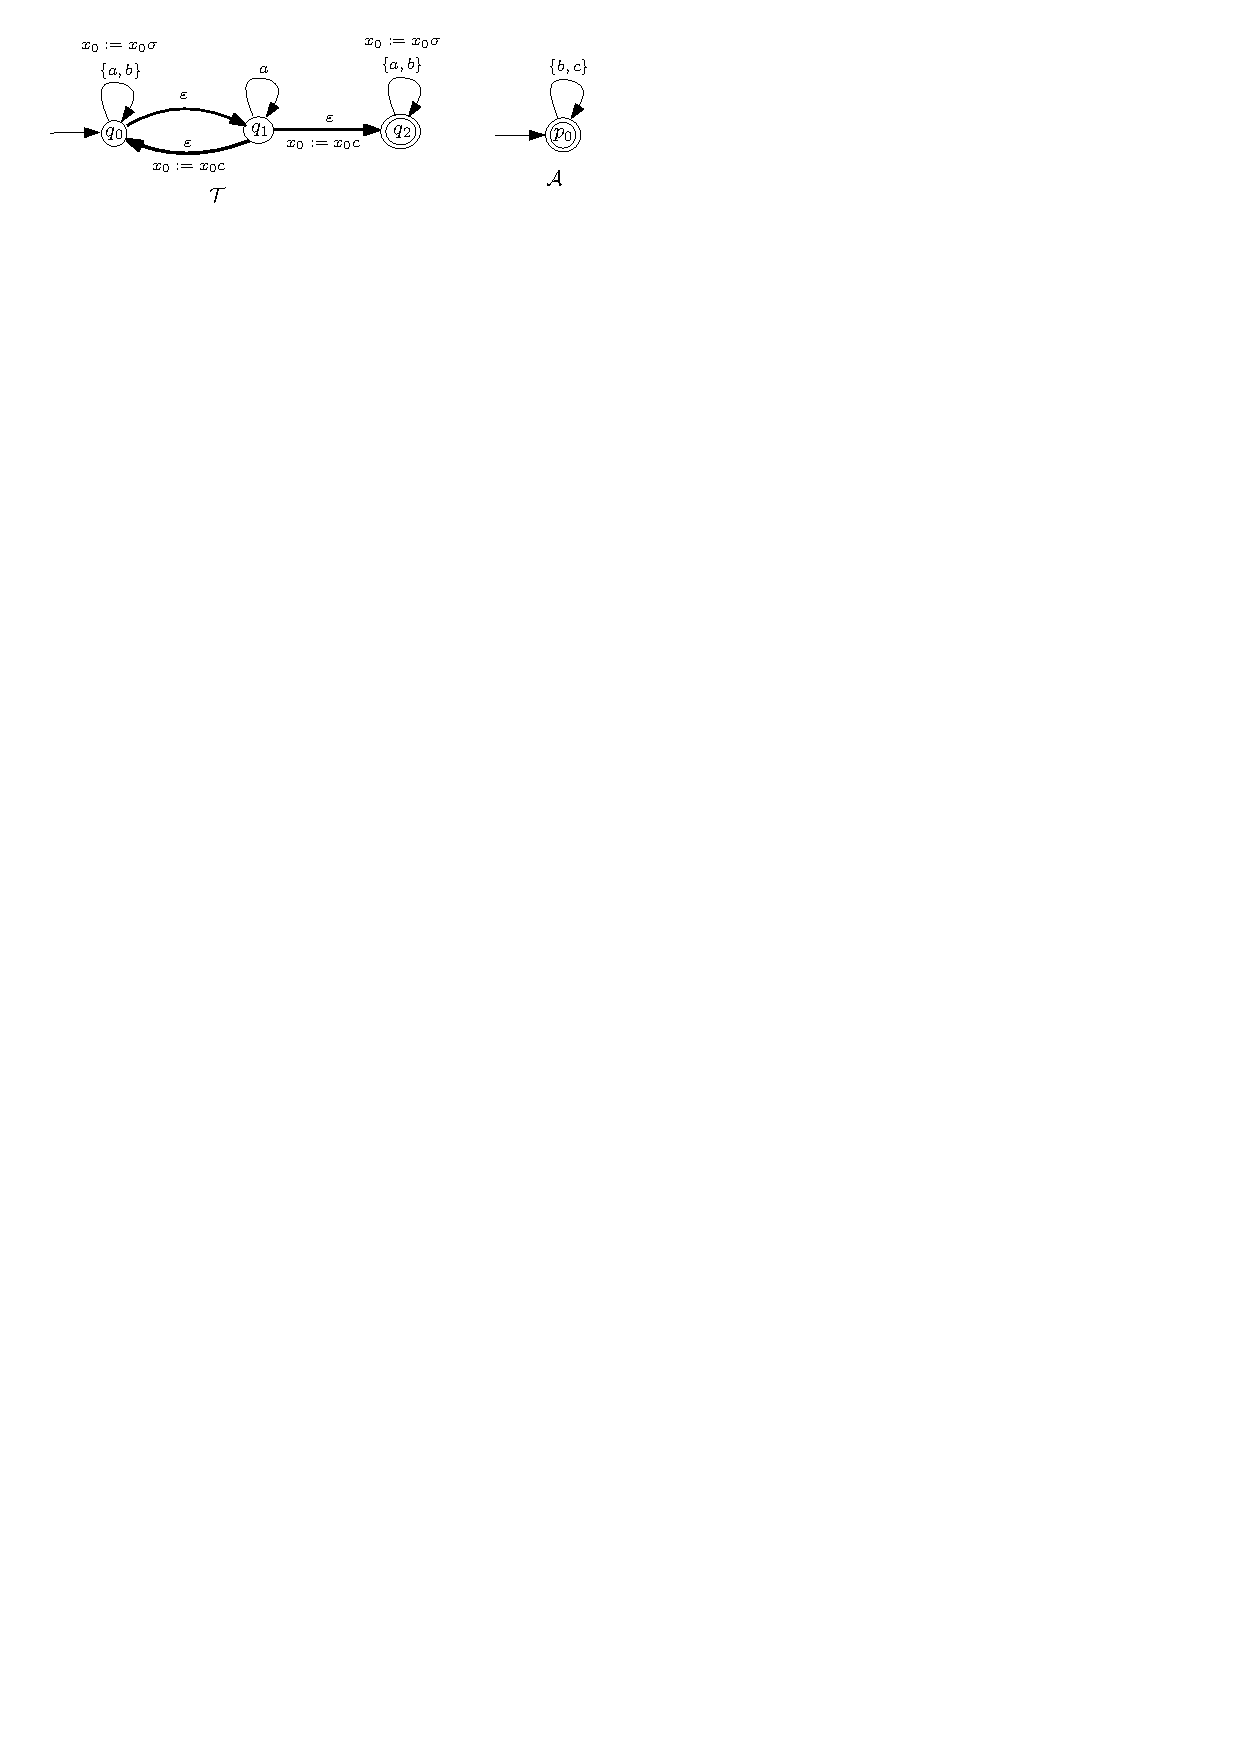
\includegraphics[scale=0.8]{pre-image-counter-example.pdf}
\caption{A counterexample to disprove the flawed pre-image construction method}
\label{fig-pre-image-count-exmp}
\end{figure}
}
%%%%%%%%%%%%%%%%%%%%%%%%%%%%%%%%
%%%%%%%%%%%%%%%%%%%%%%%%%%%%%%%%

%\begin{proof}[Lemma~\ref{lem:psst_preimage}]

%We are ready to prove Lemma~\ref{lem:psst_preimage}.

%Let $\psst = (Q_T, \Sigma$, $X, \delta_T, \tau_T, E_T,  q_{0, T}, F_T)$ be a PSST and $\Aut= (Q_A, \Sigma, \delta_A, q_{0, A}, F_A)$ be an \FA{}. 
While the aforementioned natural idea does not work,  we choose to construct an FA $\cB$ that simulates the \emph{accepting} run of $\psst$ on $w$, and, for each $x \in X$, records an $\Aut$-abstraction of the string stored in $x$, that is, the set of state pairs $(p, q) \in Q_A \times Q_A$ such that starting from $p$, $\Aut$ can reach $q$ after reading the string stored in $x$. 
To simulate the accepting run of $\psst$, it is necessary to record all the states accessible through the runs of higher priorities to ensure the current run is indeed the accepting run of $\psst$ (of highest priority). Moreover, $\cB$ also remembers the set of $\varepsilon$-transitions of $\cT$ after the latest non-$\varepsilon$-transition to ensure that no transition occurs twice in a sequence of $\varepsilon$-transitions of $\cT$.

Specifically, each state of $\cB$ is of the form $(q, \rho, \Lambda, S)$, where $q \in Q_T$, $\rho \in (\cP(Q_A \times Q_A ))^{X}$, $\Lambda \subseteq \cE(\tau_T)$, and $S \subseteq Q_T$. 
For a state $(q, \rho, \Lambda, S)$, our intention for $S$ is that the states in it are those that can be reached in the runs of higher priorities than the current run, by reading the same sequence of letters and applying the $\varepsilon$-transitions as many as possible. Note that when recording in $S$ all the states accessible through the runs of higher priorities, we do not take the non-repetition of $\varepsilon$-transitions into consideration since if a state is reachable by a sequence of $\varepsilon$-transitions where some $\varepsilon$-transitions are repeated, then there exists also a sequence of non-repeated $\varepsilon$-transitions reaching the state. 
Moreover, when simulating an $a$-transition of $\cT$ (where $a \in \Sigma$) at a state $(q, \rho, \Lambda, S)$, suppose $\delta_T(q, a) = (q_1, \cdots, q_m)$ and $\tau_T(q) = (P_1, P_2)$, then $\cB$ nondeterministically chooses $q_i$ and goes to the state $(q_i, \rho', \emptyset, S')$, where 
\begin{itemize}
\item $\rho'$ is obtained from $\rho$ and $E_T(q, \sigma, q_i)$, 
%
\item $\Lambda$ is reset to $\emptyset$,
% 
\item all the states obtained from $S$ by applying  an $a$ transition should be \emph{saturated by $\varepsilon$-transitions} and put into $S'$, more precisely, all the states reachable from $S$ by first applying an $a$-transition, then a sequence of $\varepsilon$-transitions, should be put into $S'$,
%
\item moreover, all the states obtained from $q_1,\cdots, q_{i-1}$ (which are of higher priorities than $q_i$) by saturating with $\varepsilon$-transitions should be put into $S'$,
%
\item finally, all the states obtained from those in $P'_1 = \{q' \in P_1 \mid (q, q') \not \in \Lambda\}$ (which are of higher priorities than $q_i$) by saturating with non-$\Lambda$ $\varepsilon$-transitions first (i.e. the $\varepsilon$-transitions that do not belong to $\Lambda$), and applying an $a$-transition next, finally saturating with $\varepsilon$-transitions again, should be put into $S'$, (note that according to the semantics of PSST, the $\varepsilon$-transitions in $\Lambda$ should be avoided when defining $P'_1$ and saturating the states in $P'_1$ with $\varepsilon$-transitions). 
\end{itemize}
%For technical reasons, when constructing $\cB$, we assume that this saturation happens when a state is added to $S$ for the first time. Therefore, at a state $(q, \rho, \Lambda, S)$, all the states reachable from the states in $S$ by sequences of $\varepsilon$-transitions in $\cT$ have already been in $S$.

The above construction  does not utilize the so-called \tmtextit{copyless} property (i.e. for each transition $t$ and each variable $x$, $x$ appears at most once on the right-hand side of the assignment for $t$) \cite{AC10,AD11}, 
  thus it works for general, or \textit{copyful}, PSSTs \cite{FR17}.

The formal construction of $\cB$ is omitted, due to the page limit. The interested readers can read Appendix~\ref{app-pre-image} for more details.

%%%%%%%%%%%%%%%%%%%%%%%%%%%%%%%%%%%
%%%%%%%%%%%%%%%%%%%%%%%%%%%%%%%%%%%
\hide{
\begin{table}[t]
\centering
\caption{the actual $\cB$ state in Figure 
\label{table:psst-preimage}
\ref{fig-psst-preimage-exmp}}
\begin{tabular}{|c|c|}
    \hline
    Symbol & State of $\cB$\\
    \hline
    $r_0$ & $(q_0, \rho_1, \emptyset, \emptyset)$\\
    \hline
    $r_1$ & $(q_1, \rho_1, \{ (q_0, q_1) \}, \emptyset)$\\
    \hline
    $r_2$ & $(q_2, \rho_1, \{ (q_0, q_1), (q_1, q_2) \}, \{ q_0 \})$\\
    \hline
    $r_3$ & $(q_2, \rho_2, \emptyset, \{ q_0, q_1, q_2 \})$\\
    \hline
    $r_4$ & $(q_2, \rho_1, \emptyset, \{ q_0, q_1, q_2 \})$\\
    \hline
    $r_5$ & $(q_0, \rho_1, \{ (q_0, q_1) (q_1, q_0) \}, \emptyset)$\\
    \hline
    $r_6$ & $(q_0, \rho_2, \emptyset, \emptyset)$\\
    \hline
    $r_7$ & $(q_0, \rho_2, \emptyset, \{ q_0, q_1, q_2 \})$\\
    \hline
    $r_8$ & $(q_1, \rho_2, \{ (q_0, q_1) \}, \{ q_0, q_1, q_2 \})$\\
    \hline
    $r_9$ & $(q_0, \rho_2, \{ (q_0, q_1) (q_1, q_0) \}, \{ q_0, q_1, q_2 \})$\\
    \hline
    $r_{10}$ & $(q_2, \rho_2, \{ (q_0, q_1) (q_1, q_2) \}, \{ q_0, q_1, q_2 \})$\\
    \hline
    $r_{11}$ & $(q_0, \rho_1, \emptyset, \{ q_0, q_1, q_2 \})$\\
    \hline
    $r_{12}$ & $(q_1, \rho_1, \{ (q_0, q_1) \}, \{ q_0, q_1, q_2 \})$\\
    \hline
    $r_{13}$ & $(q_0, \rho_1, \{ (q_0, q_1) (q_1, q_0) \}, \{ q_0, q_1, q_2 \})$\\
    \hline
    $r_{14}$ & $(q_2, \rho_1, \{ (q_0, q_1) (q_1, q_2) \}, \{ q_0, q_1, q_2 \})$\\
    \hline
    $r_{15}$ & $(q_2, \rho_2, \{ (q_0, q_1) (q_1, q_2) \}, \{ q_0 \})$\\
    \hline
    $r_{16}$ & $(q_1, \rho_2, \emptyset, \{ q_0, q_1, q_2 \})$\\
    \hline
    $r_{17}$ & $(q_2, \rho_2, \{ (q_1, q_2) \}, \{ q_0, q_1, q_2 \})$\\
    \hline
    $r_{18}$ & $(q_0, \rho_2, \{ (q_1, q_0) \}, \{ q_0, q_1, q_2 \})$\\
    \hline
    $r_{19}$ & $(q_1, \rho_2, \{ (q_1, q_0) (q_0, q_1) \}, \{ q_0, q_1, q_2 \})$\\
    \hline
    $r_{20}$ & $(q_2, \rho_2, \{ (q_1, q_0) (q_0, q_1) (q_1, q_2) \}, \{ q_0, q_1, q_2 \})$\\
    \hline
    $r_{21}$ & $(q_1, \rho_2, \{ (q_0, q_1) \}, \emptyset)$\\
    \hline
    $r_{22}$ & $(q_0, \rho_2, \{ (q_0, q_1) (q_1, q_0) \}, \emptyset)$\\
    \hline
\end{tabular}
\end{table}
}
%%%%%%%%%%%%%%%%%%%%%%%%%%%%%%%%%%%
%%%%%%%%%%%%%%%%%%%%%%%%%%%%%%%%%%%

%
%\zhilin{stopped here}
%\zhilei{changed a little bit}

%%%%%%%%%%%%%%%%%%%%%%%%%%%%%%%%%%%%%%%%%
%%%%%%%%%%%%%%%%%%%%%%%%%%%%%%%%%%%%%%%%%
\hide{
\subsection{Complexity}

\begin{proposition}[POPL'19]
	The path feasibility problem of the following two fragments is non-elementary: SL with 2FTs, and SL with FTs+replaceAll.
	
	SL[conc, replaceAll, reverse, FFT] is expspace-complete (note that 2FTs in SL are restricted to be one-way and functional)
\end{proposition}

%The same proof strategy can be used for FTs+replaceAll. The 2FTs used in the proof above
%proceed by running completely over the word and producing some output, then silently moving
%back to the beginning of the word. An arbitrary number of passes are made in this way. We
%can simulate this behaviour using FTs and replaceAll.


The main open question is the complexity of the SL fragment with replaceall function and prioritized streaming transducers. Note that PSST can simulate 2FT (adapting Matt's proof?), so we could obtain nonelementary lower bound for SL with PSST.

However, this variant of replaceall is quite different from the replaceall we had before ...

\begin{enumerate}
\item  does  copyless help?
\item how about SL with only this version of replaceall?
\end{enumerate}
}
%%%%%%%%%%%%%%%%%%%%%%%%%%%%%%%%%%%%%%%%%
%%%%%%%%%%%%%%%%%%%%%%%%%%%%%%%%%%%%%%%%%
